\setlength{\columnsep}{2pt}
\setlength{\columnseprule}{0pt}
\begin{multicols}{2}
	Η μεταβολή του ρεύματος στη βάση του transistor επιτυγχάνεται μέσω της μεταβολής της τάσης στην έξοδο της γεννήτριας. Η εναλλασσόμενη πηγή τάσης \texttt{Vce} έχει περίοδο $T_{v_{CE}}=\sfrac{1}{1\unit{\kilo\hertz}}=1\unit{\milli\second}$ αρκετά μικρότερη από την διάρκεια κάθε βήματος της γεννήτριας, $t_s=$. Επομένως, το ρεύμα στη βάση του transistor παραμένει σταθερό για αρκετό χρόνο ώστε να ολοκληρωθεί η σάρωση της διαφοράς δυναμικού μεταξύ συλλέκτη και εκπομπού.\par
	Η προσομοίωση γίνεται στο πεδίο του χρόνου σε διάστημα μίας περιόδου της κλιμακωτής τάσης. Μέσω των ρυθμίσεων των αξόνων στο PSpice, επιλέγεται η διαφορά δυναμικού μεταξύ συλλέκτη και εκπομπού ως η μεταβλητή του οριζόντιου άξονα. Ως \texttt{trace} του γραφήματος επιλέγεται το ρεύμα στον εκπομπό. Τα αποτελέσματα της προσομοίωσης φαίνονται στο διάγραμμα \ref{plot:2_bjt}.\par
	\begin{center}
		\begin{circuitfig}[H]
			\centering
			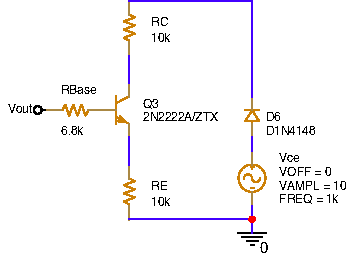
\includegraphics[width=5cm]{spice_02/ask2_bjt_schematic.pdf}
			\caption{Κύκλωμα για τη λήψη των χαρακτηριστικών $v_{CE}-i_C$ ενός BJT. Το κύκλωμα συνδέεται στην έξοδο της γεννήτριας κλιμακωτής τάσης.}
			\label{circ:2_bjt_schematic}
		\end{circuitfig}
	\end{center}
\end{multicols}
\vspace*{-0.35cm}
\begin{plot_fig}[H]
	\begin{center}
		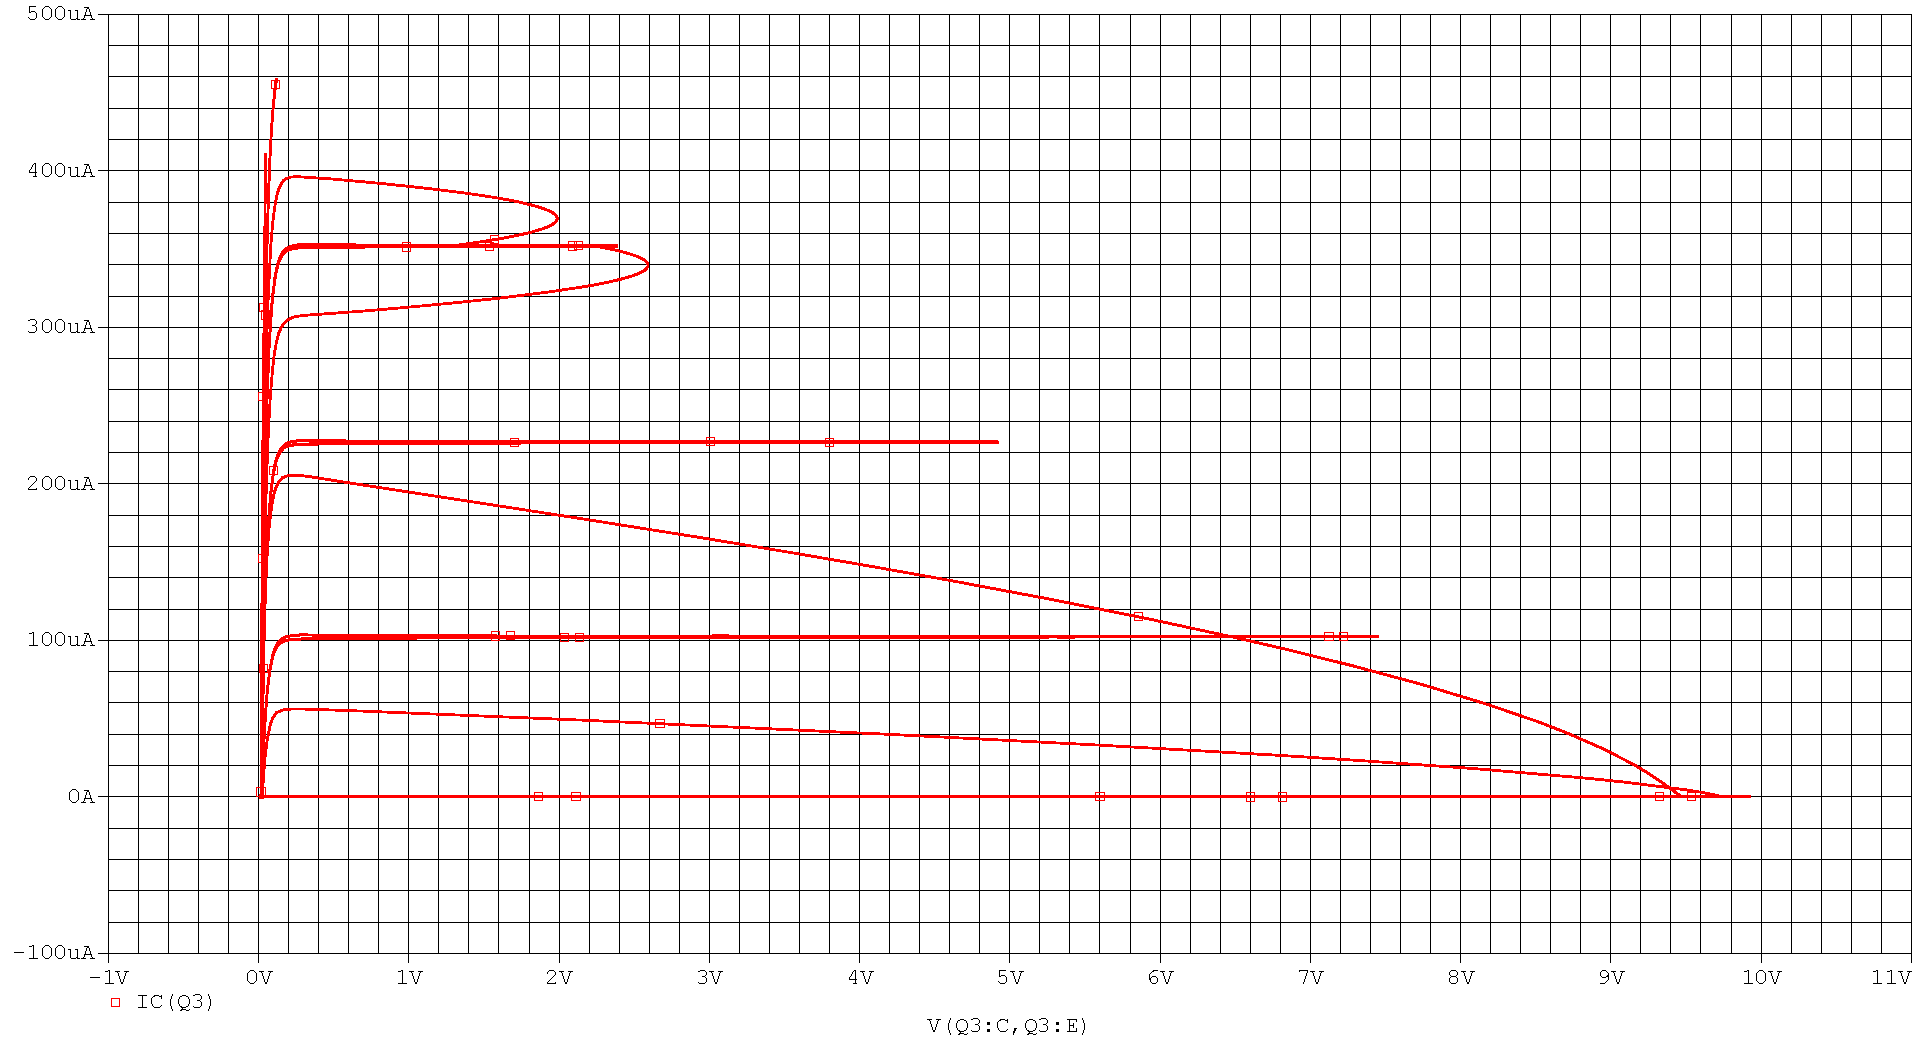
\includegraphics[height=5.5cm]{spice_02/q6.pdf}
		\caption{Χαρακτηριστικές $v_{CE}-i_C$. Οι \textsl{ενδιάμεσες} καμπύλες, μεταξύ των αναμενόμενων καμπυλών, οφείλονται στο γεγονός πως καθώς μεταβάλλεται η έξοδος της γεννήτριας η σάρωση της πηγής \texttt{Vce} του κυκλώματος \ref{circ:2_bjt_schematic} συνεχίζεται.}
		\label{plot:2_bjt}
	\end{center}
\end{plot_fig}